\documentclass[12pt]{beamer}

%% Based on the original theme by Matthias Vogelgesang

\usetheme[progressbar=frametitle]{metropolis}
\usepackage{appendixnumberbeamer}

\usepackage{booktabs}
\usepackage[scale=2]{ccicons}


\usepackage{graphicx,threeparttable,caption}

%\usepackage{pgfplots}
%\usepgfplotslibrary{dateplot}

% \usepackage{background}
% \backgroundsetup{
%     placement=center,
%     scale=8,
%     contents={DRAFT},
%     opacity=1.5
% }
% \setbeamertemplate{background}{\BgMaterial}

\usepackage{xspace}
\newcommand{\themename}{\textbf{\textsc{metropolis}}\xspace}

\usepackage[style=apa, sortcites=true, sorting=nyt, backend=biber]{biblatex}
\DeclareLanguageMapping{american}{american-apa}

\usepackage[export]{adjustbox}
\usepackage{graphicx}
\graphicspath{ {./images/} }

\usepackage{threeparttable}


%% adding bibliography file to list of resources
\addbibresource{bibliography.bib}


%%%%%%%%%%%%%%%%%%%%%%%%%%%%
%% UNCC Theme Adjustments %%
%%%%%%%%%%%%%%%%%%%%%%%%%%%%
\definecolor{CanvasBG}{HTML}{FAFAFA}

% From the official style guide
\definecolor{UnccGreen}{HTML}{00703C}
\definecolor{UnccGold}{HTML}{B3A369}
\definecolor{UnccLightGreen}{HTML}{C3D7A4}
\definecolor{UnccYellow}{HTML}{F0CB00}
\definecolor{UnccOrange}{HTML}{F3901D}
\definecolor{UnccLightYellow}{HTML}{FFF6DC}
\definecolor{UnccBlue}{HTML}{00728F}
\definecolor{UnccPink}{HTML}{DE3A6E}
\definecolor{White}{HTML}{FFFFFF}
\definecolor{LightGray}{HTML}{DDDDDD}

% Supporting Color Palette
\definecolor{WarmGray}{HTML}{696158}
\definecolor{StoneGray}{HTML}{717C7D}
\definecolor{DarkGreen}{HTML}{2C5234}
\definecolor{LightGreen}{HTML}{509E2F}
\definecolor{BrightGold}{HTML}{F0CB00}

% Screamers
\definecolor{Royal}{HTML}{72246C}
\definecolor{Ocean}{HTML}{006BA6}
\definecolor{Flash}{HTML}{B52555}
\definecolor{Citrus}{HTML}{FFB81C}
\definecolor{Spring}{HTML}{CEDC00}

% Serenity
\definecolor{Garden}{HTML}{B7CE95}
\definecolor{Sand}{HTML}{F0E991}
\definecolor{Bloom}{HTML}{F1E6B2}
\definecolor{Clay}{HTML}{B7B09C}
\definecolor{Cloud}{HTML}{BAC5B9}

% Set colors here
\setbeamercolor{frametitle}{bg=UnccGreen}
\setbeamercolor{progress bar}{bg=BrightGold, fg=UnccGreen}
\setbeamercolor{alerted text}{fg=Flash}

\setbeamercolor{block title}{bg=LightGreen, fg=White}
\setbeamercolor{block title example}{bg=Ocean, fg=White}
\setbeamercolor{block title alerted}{bg=Citrus, fg=White}
\setbeamercolor{block body}{bg=CanvasBG}

\metroset{titleformat=smallcaps, progressbar=foot}

\makeatletter
\setlength{\metropolis@progressinheadfoot@linewidth}{2pt}
\setlength{\metropolis@titleseparator@linewidth}{2pt}
\setlength{\metropolis@progressonsectionpage@linewidth}{2pt}
%%%%%%%%%%%%%%%%%%%%%%%%%%%%
%% UNCC Theme Adjustments %%
%%%%%%%%%%%%%%%%%%%%%%%%%%%%


\title{Sprint 2}
\subtitle{College and Career Readiness in Charlotte, NC: An Analysis on Academic Performance, Career Readiness, and Upward Mobility.}
% \date{\today}
\date{February 9, 2022}
\author{Khem Khadka \and Cody Scott \and Joshua Hernandez}
\institute{DTSC 4301 \\ School of Data Science \\ University of North Carolina at Charlotte}
%\titlegraphic{\vspace{4.5cm}\flushright}%\includegraphics[height=3cm]{UNC_Logo.png}}
\usepackage[sfmath]{kpfonts}


\begin{document}


\maketitle

\begin{frame}{Table of contents}
  \setbeamertemplate{section in toc}[sections numbered]
  \tableofcontents[hideallsubsections]
\end{frame}

\section[Overview]{Overview}

\begin{frame}[fragile]{Project Overview}
    \begin{itemize}
        \item chetty
        \item LOO
        \item Will fill this out when draft is done
    \end{itemize}
\end{frame}

\subsection[Research Question]{Research Question}

\begin{frame}{Research Question}
    \large{\textsc{Will the recommendations made from the task force show a positive effect on minority children, and children from low economic statuses in educational performance, college readiness, or career readiness?}}

\end{frame}

\section[Hypotheses]{Hypotheses}

\begin{frame}[fragile]{Hypotheses}

    \begin{block}{Hypothesis 1}
        As the number and quality of mentors increase, there will be an increase in academic performance and college acceptance rates for low-socioeconomic students.
    \end{block}

    \pause

    \vspace{1cm}

    \begin{exampleblock}{Variables}
        \begin{itemize}
            \item[$\triangleright$] AP Participation Rate
            \item[$\triangleright$] AP Passing Rate
            \item[$\triangleright$] College Enrollment Rate 
            \item[$\triangleright$] Total Guidance Counselors in Charlotte-Mecklenburg Schools
            \item[$\triangleright$] Quality of Mentor Bias Training
        \end{itemize}
    \end{exampleblock}

\end{frame}

\begin{frame}[fragile]{Hypotheses}

    \begin{block}{Hypothesis 2}
        As the quality of mentors and counselors increase, there will be an increase in obtained CTE  Credentials by students within Charlotte Mecklenburg County Schools.
    \end{block}

    \pause 

    \vspace{1cm}

    \begin{exampleblock}{Variables}
        \begin{itemize}
            \item[$\triangleright$] Career and Technical Education Enrollment
            \item[$\triangleright$] Career and Technical Education Credentials
            \item[$\triangleright$] Total Guidance Counselors in Charlotte-Mecklenburg Schools
            \item[$\triangleright$] Quality of Mentor Bias Training
        \end{itemize}
    \end{exampleblock}

\end{frame}

\begin{frame}[fragile]{Hypotheses Model}

%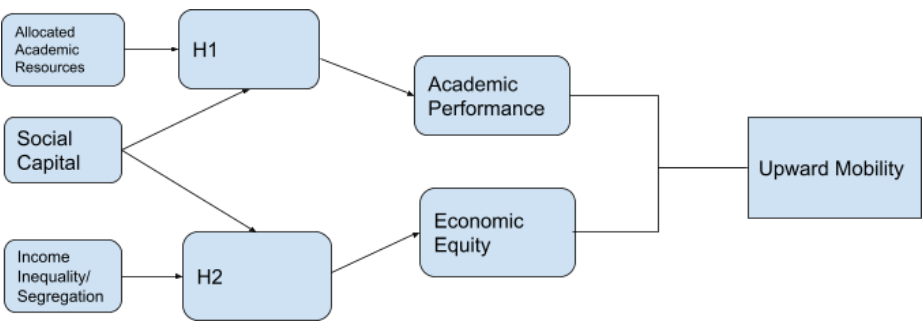
\includegraphics[width=11.4cm]{Hypothesis Model.png}

\end{frame}


\section[Data Sources]{Data Sources}

\begin{frame}{Data Sources}

    \begin{exampleblock}{Sources}
        \begin{itemize}
            \setlength\itemsep{3mm}
            \item[$\triangleright$] North Carolina Department of Public Instruction
                \begin{itemize}
                    \item North Carolina School Report Cards
                    \item North Carolina Public Schools Statistical Profile
                    \item The Educational Directory and Demographical Information Exchange (EDDIE)
                \end{itemize}
            \item[$\triangleright$] The National Center for Education Statistics 
                \begin{itemize}
                    \item Education Demographics and Geographic Estimates on School Neighborhood Poverty
                \end{itemize}
            \item[$\triangleright$] Charlotte Open Data Portal
                \begin{itemize}
                    \item 2019 Median Household Income by school Zip Code
                \end{itemize}
        \end{itemize}
    \end{exampleblock}

\end{frame}


\section[Variable Information]{Variable Information}


\begin{frame}{Codebook}
    table here
\end{frame}


\begin{frame}{Summary Statistics}
    table here
\end{frame}

\section[Analysis and Validation]{Analysis and Validation}

\begin{frame}{Potential Analysis}
    info
\end{frame}

\begin{frame}{Hypothesis Validation}
    info
\end{frame}

\begin{frame}{Next Steps}
    info
\end{frame}




{\setbeamercolor{palette primary}{fg=black, bg=yellow}
\begin{frame}[standout]
  Questions?
\end{frame}
}


\end{document}
